\chapter{State of the Art}
\label{chapter:state_of_the_art}

This chapter aims to provide a description and overview of important concepts of Fault Tolerance in Component-based Systems, \ac{bas}, \ac{iot} as well as event processing. For each topic there will be a review of the different technologies and protocols, how they interact and how they differ from each other.

All of the topics addressed in this chapter contributed to the solution presented, either in a combination of different technologies or choosing from similar ones.


\section{Fault Tolerance in Component-based Systems}

Nowadays, most system architectures are composed by individual components(physical or logical) with well-defined communication interfaces. This can bring several advantages such as the reusability or replaceability of components without affecting the overall functioning of the system \cite{TutorialsPoint}.

Nevertheless, this type of architecture has to be tolerant to failures of components(or nodes), in order to achieve an high availability solution, which is a crucial feature to the majority of systems \cite{Sun2014a}. As the author of \cite{Zaiter2013} suggests, an error is the manifestation of a fault in the system, and a failure is the manifestation of an error on the provided service by the system. The same author also classify the faults on the base of the faults’s sources, their manifestations and their persistence, namely software errors, materials errors or transmission errors. Therefore a node failure can be caused either by an internal error on the software, a physical malfunctioning on the component or the shutdown of the communication links to the node.

In order to have a fault tolerant system, there must be implemented fault detection and fault recovery techniques. Bellow, will be presented some of those techniques.

\begin{Paragraph}{Fault Detection Techniques}
	
	Fault detection is the process of collecting information about the system's nodes state. This information can be gathered by failure detectors using two different keep alive messages: ping and heartbeat \cite{Zaiter2013}. In the first one the failure detector sends a ping message to the monitored nodes and waits to receive an acknowledge message. If the monitored node is down, due to a failure, the failure detector will not receive the \textit{ack} and therefore conclude that the node is down. The last one, the heartbeat message, in contrast to the ping message, it is the monitored nodes that send a periodic message to the failure detector, informing that it is still running as expected. If the detector does not receive a heartbeat message from a node, after a timeout, it concludes that the node is no longer available. The author of \cite{Zaiter2013}, claims that heartbeat messages have more advantages when compared to ping messages, such as the heartbeat need of half the messages used by ping detectors. However, the ping detectors only have to preform time control in case of a failure in receiving an acknowledge, while the heartbeat detectors need to keep track of the time to detect the absence of heartbeats after a timeout. 
	
	Regarding the fault detector location in the system, the author of \cite{kshir} identifies two approaches, a centralized or distributed detector. The centralized approach uses a single node to preform the monitoring of other components, however, although this approach being efficient and accurate to identify faults \cite{kshir}, it constitutes a single-point of failure in the system. Plus, in large-scale systems, the messages traffic can congest the network which can result in a more expensive and inefficient solution. The distributed approach uses several nodes as failure detectors, which eliminates the single-point of failure problem, however, introduces much more complexity to the system \cite{Zaiter2013}. 
	
	
\end{Paragraph}

\begin{Paragraph}{Fault Recovery Techniques}

The fault recovery occurs immediately after a detector sense the fault of a system's node. According to the author of \cite{Schweiz}, the high availability of a system is normally achieved using redundant entities, whereby, when a component fails, the redundant node takes over its tasks. The author of \cite{Redwine} states that there are two types of physical redundancy: active replication and primary backup. 

Regarding the active replication, it is usually addressed as a N-modular redundancy approach \cite{Schweiz}, in which a set of replicated modules receive the same input, and the resulting outputs from the different modules are compared and the result with more concordance(majority) is elected as the output. In Figure \ref{fig:nmodular} is represented this active replication method. The most common N-modular redundancy is the \acf{tmr}. \ac{tmr} uses a set of three replicated modules, thus, it allows that a module can fail, or produce a faulty value, and, the other correctly working modules, are able to mask that failure. 
	
	\begin{figure}[H]
		\centering
		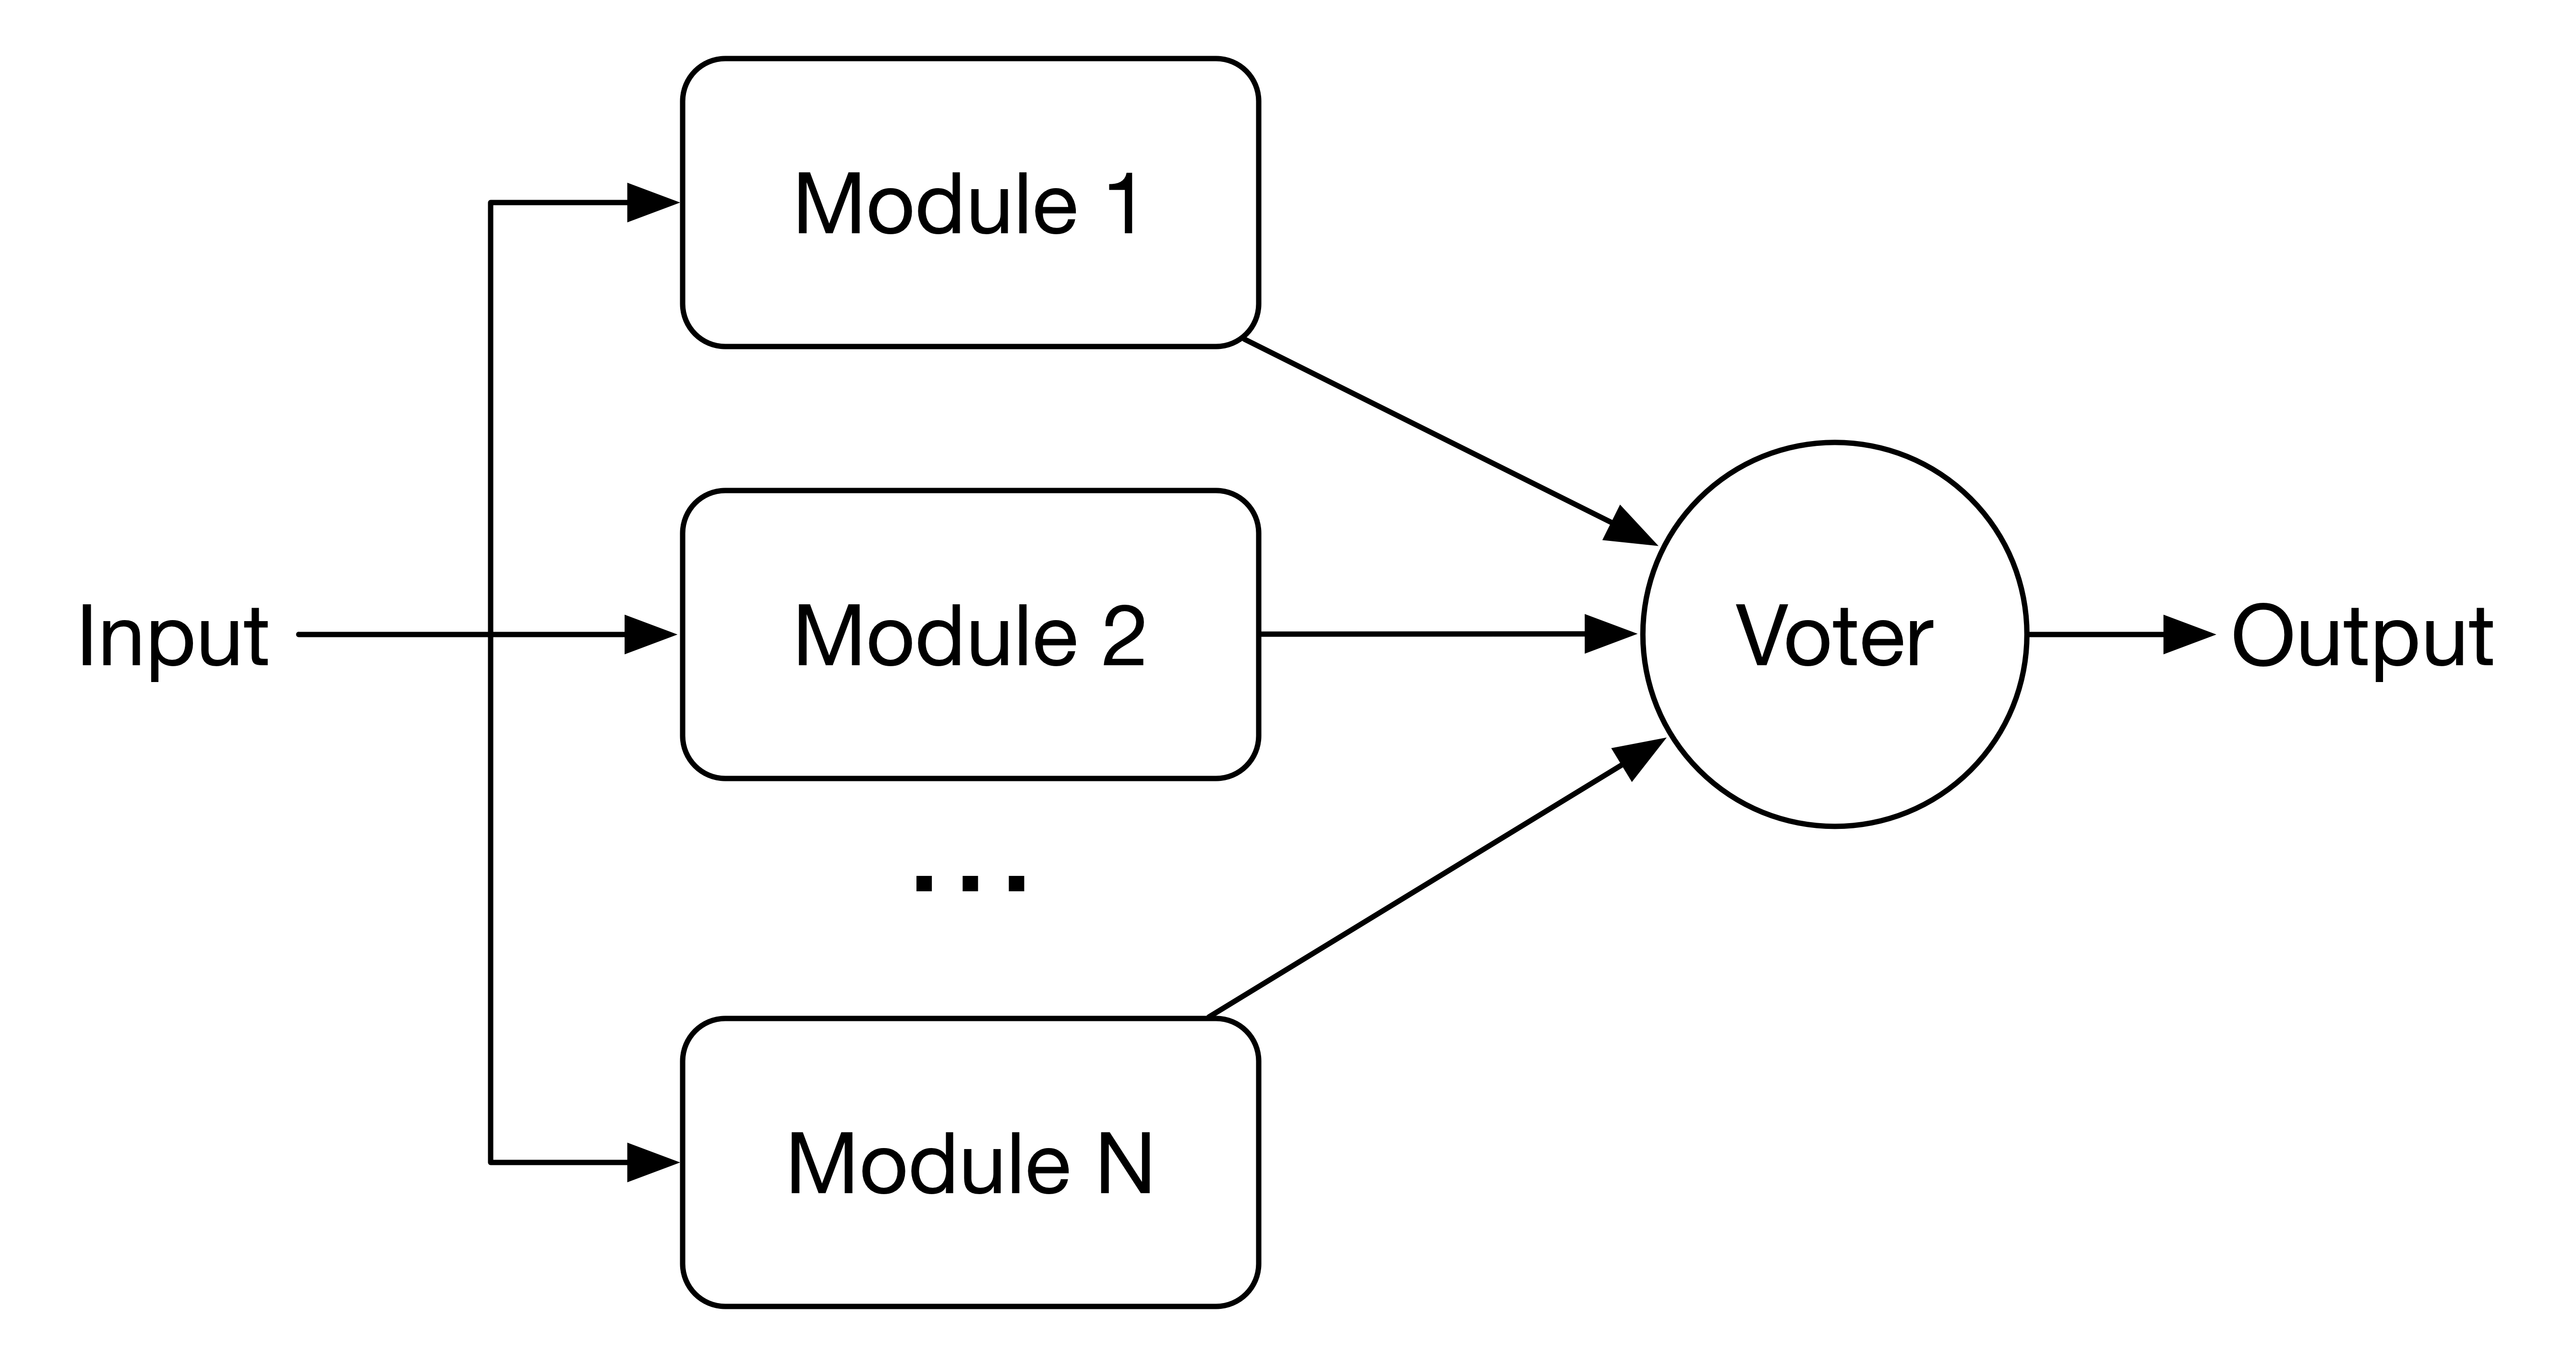
\includegraphics[width=0.7\textwidth]{figures/nmodular.png}
		\caption{N Modular Redundancy.}
		\label{fig:nmodular}
	\end{figure}

Concerning the primary backup approach, also known as hot standby redundancy \cite{Schweiz}, it uses a primary node, and one or more unused backup nodes. In this approach, there is a need for a failure detector so that when the primary node fails, the backup node can be notified to take over the processing. In Figure \ref{fig:hot_standby} it is represented the hot standby redundancy, and as can be observed, both the active and the passive replicated module need to be connected in order to be synchronized \cite{Schweiz}. 

	\begin{figure}[H]
		\centering
		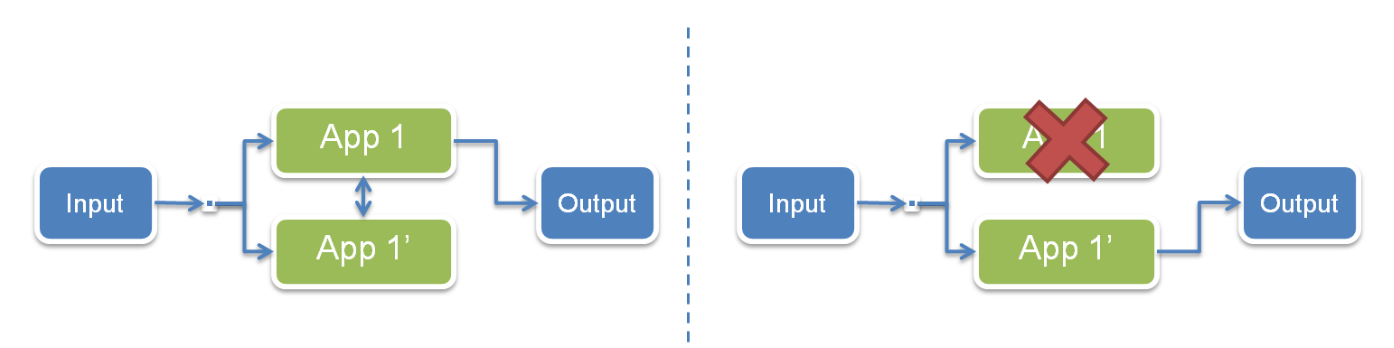
\includegraphics[width=0.9\textwidth]{figures/hotstandby.png}
		\caption{Hot standby redundancy. Adapted from \cite{Schweiz}.}
		\label{fig:hot_standby}
	\end{figure}

The author of \cite{Schweiz} also states, as an example, a situation with three hosts connected through a common communication bus. Each host need to send periodic heartbeat messages to this bus and, if a host's heartbeat is missing, due to a failure in the host or in the network, the other hosts can act immediately to resolve the failure.
	
\end{Paragraph}

The methods presented in this chapter can be used in any component-based system to achieve an acceptable level of fault tolerance, however, each method can be more suitable to different situations. Over the next chapters, this methods will be evaluated in more specific areas like \acf{wsn}s and \acf{bas}s. 

\section{Building Automation System}

A Building Automation System consists in the automatic control and monitoring of building services such as lighting, heating, ventilation, air conditioning, and more. The main purpose of \ac{bas} is to improve the comfort of the building's occupants, while significantly decreasing the operational costs and energy consumption. This is achieved using the information gathered by a wide set of sensors, that is used to control building equipment behaviour such as lighting, \ac{hvac}, shutters, and others \cite{Brambley2005}. This information can also be used to prevent and react quickly to emergency situations, allowing to resolve them with minimum or even non human intervention.

\begin{figure}[H]
	\centering
	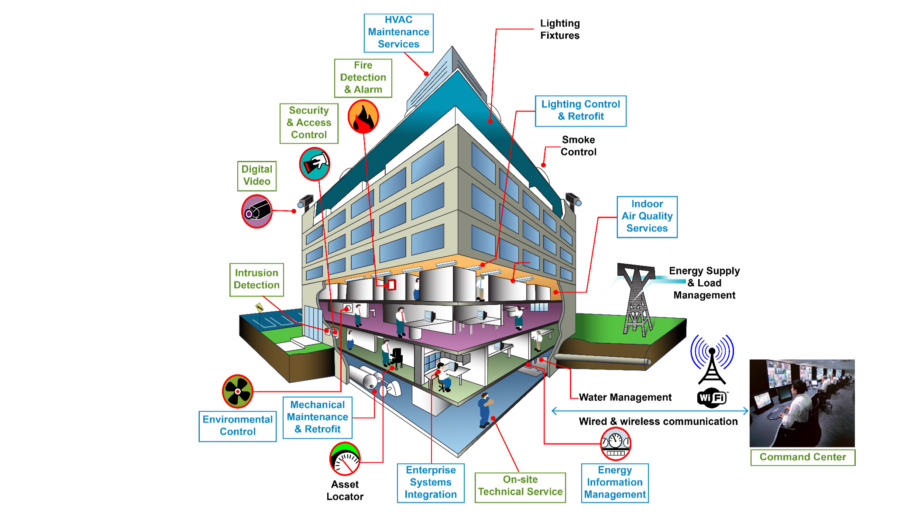
\includegraphics[width=0.9\textwidth]{figures/smart-building.jpg}
	\caption{Building Automation System schematic. Adapted from \cite{image-BAS}. }
	\label{fig:smart-building}
\end{figure}

The biggest problem in building automation is the market segmentation, where different manufactures created over the years different protocols and communication standards that didn't address solutions to all types of applications. This led to a more difficult and often impossible integration of this different approaches in the same system. Also, each vendor used to have closed specifications but, recently, in order to gain a higher margin of market, this specifications started being disclosed by vendors, which led to the appearence of new standards made from prior ones, combined. Presently, the most common communication and management standards used in BAS are \acf{bacnet} \cite{bacnet}, \acf{knx} \cite{knx}, \acf{lonworks} \cite{EchelonCorporation2009}, and \acf{dali} \cite{dali}.  Each one of them as an important role at different levels of a Building Automation System. As shown in Figure \ref{fig:hierarchy}, those levels are Management System Level, Automation Level and Field Level \cite{Iwayemi2011}. The all set of devices, sensors or actuators, compose the field layer. The Automation level is responsible for all the logic and hardware needed to control those devices and the Management Level consists in the control and management of the system and the reactions to events present in the gathered data.

\begin{figure}[H]
	\centering
	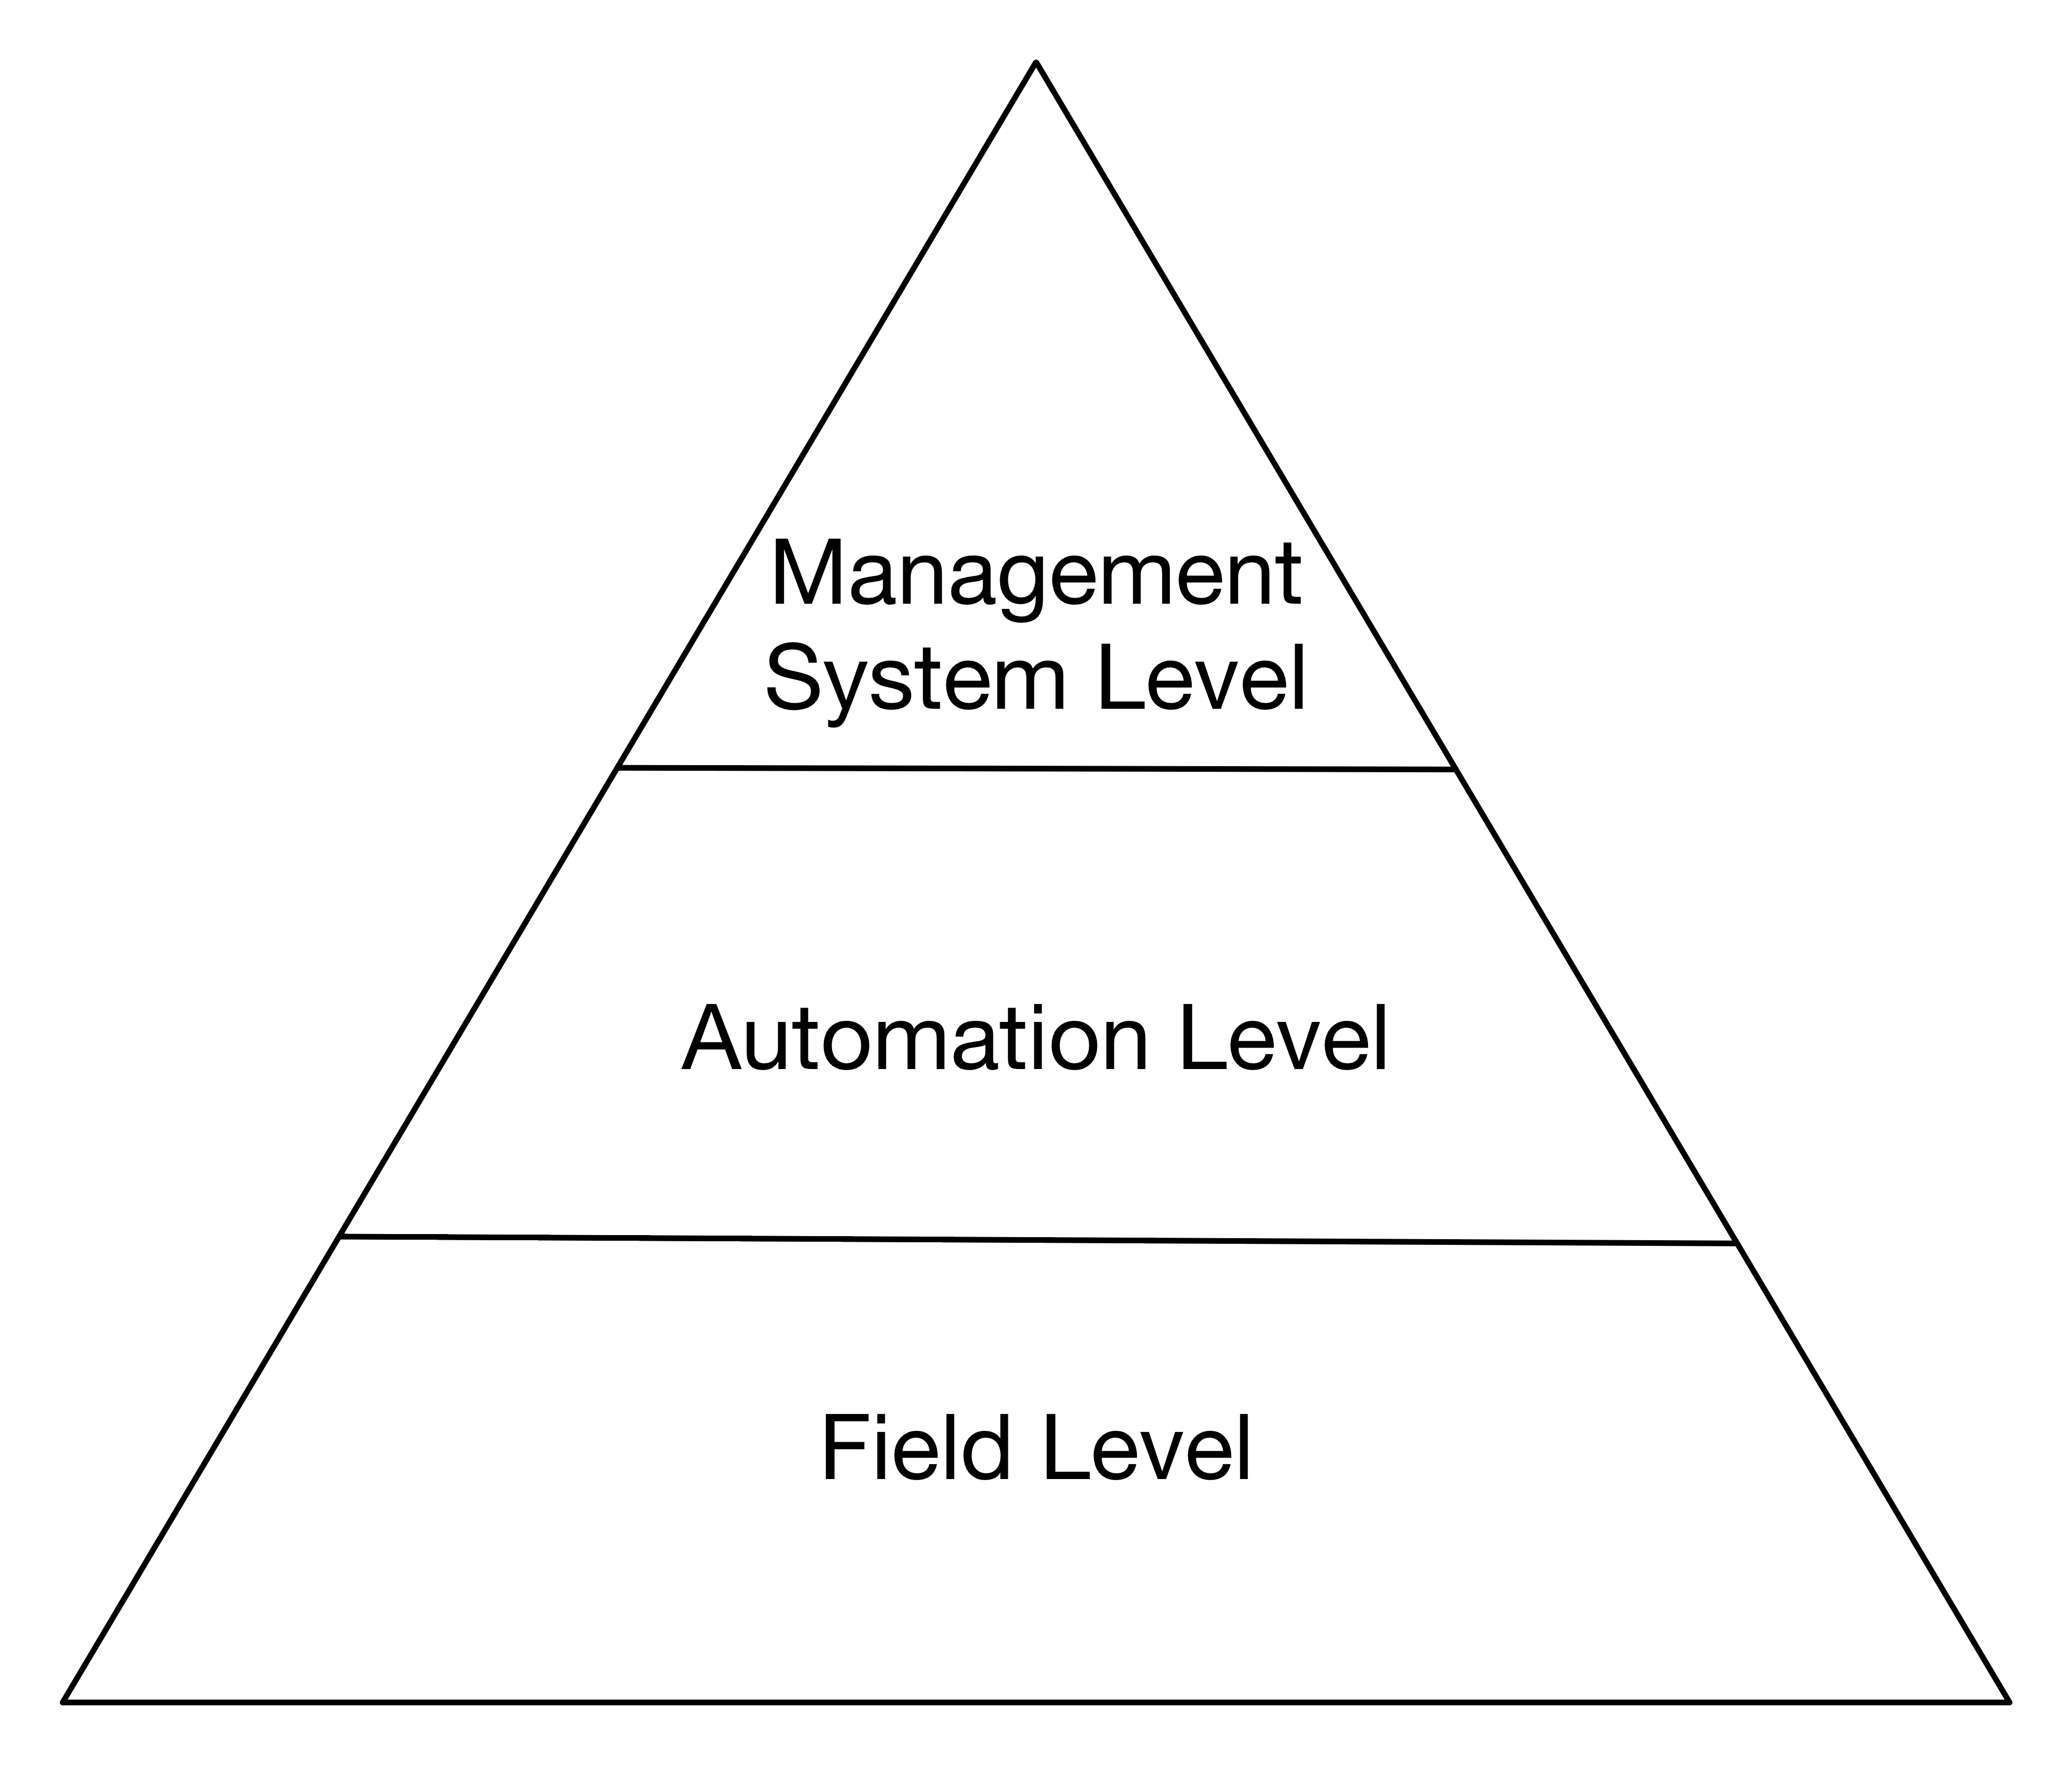
\includegraphics[width=0.6\textwidth]{figures/hierarchy.png}
	\caption{Building Automation System hierarchy \cite{kastener}. }
	\label{fig:hierarchy}
\end{figure}

Regarding the most used standards, all excepting \ac{dali}, which is a standardized interface for lighting control and a Field level only protocol, allow communication of building automation and control systems in fields such as HVAC, lighting control and others \cite{Siemens2013}. The other three protocols actuate at the Automation level, being \ac{knx} also in the Field level and \ac{bacnet} in the Managemet System level.



\subsection{\ac{bas} Solutions}

Over the years a large number of companies step forward to offer solutions for reducing energy consumption in buildings. Companies like Siemens, which provides three different \ac{bas} systems, Honeywell, and Johnson Controls, which claims to be the leader of the building automation market, offer services, using, most of the times, the formerly addressed open standard protocols.

However, this products have some common drawbacks: most of them are highly costly, which ends up to be a problem for medium to small companies to afford, and also, the most important of all, are not open source and don't allow for building managers to install and integrate new devices and feature at will. 

Though, with the rising of \ac{iot}, there have been an increasingly amount of new solutions that use high scalable technologies, well known communication standards, such as IP,  and use lightweight devices with low power consumption. This concepts will be addressed over the next section

\section{\acf{iot}}

\acf{iot} is a concept that have been emerging over the years in which in addition to the devices we usually connect to the Internet, like smartphones or personal computers, a new diversity of devices will also be connected, forming a vast network of smart objects. Devices like vehicles or normal household appliances will be equipped with sensors and actuators that will be able to gather data, giving people the information to do better and valuable decisions \cite{Weiser1991}. Also, with controllers and the sensing information, these devices can preform certain tasks without human intervention. There was already a concept, used in telemetry, industrial and automation systems, \acf{m2m}, which enabled the exchange of information between machines, in order to perform tasks and actions without human intervention. Although both of the concepts goals remain alike, i.e. enable communication between machines, \ac{m2m} should be considered as a subset of \ac{iot}, as it lacks in the creation of meaning to the information exchanges.

The concept of \ac{iot} was first introduced by Kevin Ashton \cite{Ashton} in 1999, where he stated his idea of having computers gathering information from things around us, that humans couldn't do by themselves, to give a new perspective to people of how to reduce waste, loss and cost. For this author, we needed to give computers the power to gather information with their own means, so they could sense the world for themselves and overcome the limited time, attention and accuracy humans have.

In the recent years, with the technological advances made in electronics, devices become smaller, low powered and more affordable, giving a boost to the integration of this concept in our society. According to \cite{Evans2011}, the turning point for \ac{iot} would be when there were more devices connected to the Internet than people. This point was reached somewhere between 2008 and 2009, and as can be seen in Figure \ref{fig:iot_pic}, this numbers will grow exponentially in the next years and can even reach over a 5 to 1 factor between connected devices and the world population.

\begin{figure}[H]
	\centering
	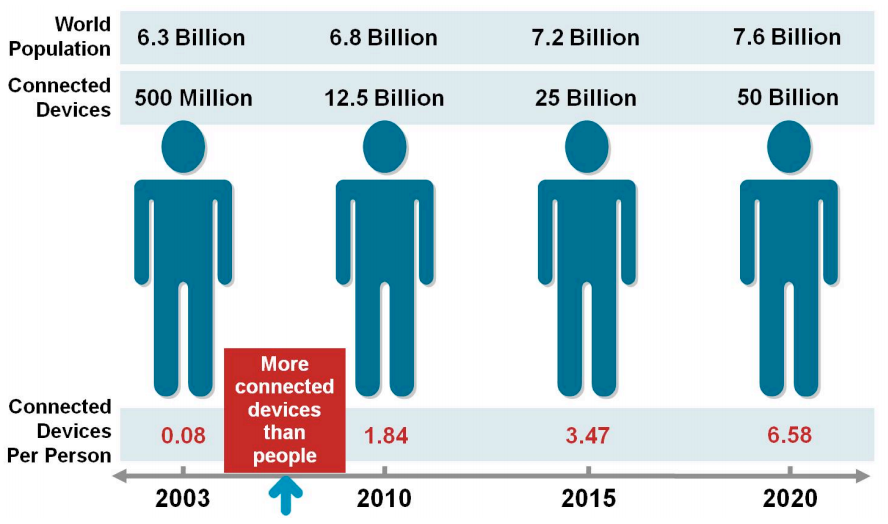
\includegraphics[width=0.9\textwidth]{figures/iot_pic.png}
	\caption{Estimated growth of connected devices \cite{Evans2011}. }
	\label{fig:iot_pic}
\end{figure}

\acf{m2m} term firstly emerged a few decades ago and it was used in telemetry, industrial and automation systems \cite{}. Nowadays it is often associated with \ac{iot}, since it refers to the exchange of information between machines, in order to preform tasks and actions without human intervention.

Although both of the concepts goals remain alike, i.e. enable communication between machines, \ac{m2m} should be considered as a subset of \ac{iot}, as it lacks in the creation of meaning to the information exchanges. \ac{iot} is a wide web of not only \ac{m2m} networks but also, a vast set of applications that enables, as stated in the previous section, automatic decision making and data analytics. 

Nevertheless, the growth of \ac{iot} still faces some challenges. As the authors of \cite{Al-fuqaha2015} state, with the grow number of devices being connected to the Internet, IPv6 is going to be crucial for the billions of new devices that will require for a unique IP address. The devices will also need to be self-sustainable with regard to energy consumption. Besides this factors, \ac{iot} remains with no agreements on what standards should be used, which is a problem since it hampers the communication between devices


The \ac{iot} concept, according to \cite{Evans2011} will be a very important evolution to the Internet, giving the ability to create new applications to improve people's lives. The sharing of knowledge and wisdom has always been a key factor for human evolution, and now, with \ac{iot} and the help of smart devices that sense, collect and share information, we can create new ways to enhance people's comfort and well-being.

\ac{iot} will have an important role in a vast number of sectors, and Building Automation is an example of that. The IoT's rapid growth is giving building managers a wide variety of new technology choices. Darcy Otis, director of analytics and fault detection for the building technologies division at Siemens states that IoT will give BAS more information and better tools to perform its core functions\cite{biot}.


\subsection{\acf{wsn}}

\acf{wsn} is a network of distributed devices, sensors and/or actuators, interconnected by a wireless medium. As stated in \cite{IEC2014a}, this network of nodes sense and control the environment cooperatively, enabling the interaction between persons or computers and the environment around them. 

Nowadays \ac{wsn}s usually include sensors, actuators and gateways. Sensors are devices capable of detecting changes in environmental variables and supply that information to other nodes. This devices can measure variables like luminosity, temperature, humidity, pressure, motion and a wide variety of other environmental data. Actuators, in the other hand, are devices that control mechanisms to alter the physical environment state and preform this actions based on input data. For instance, an actuator can be programmed to turn on or off a air conditioner based on a input trigger set off by the temperature in a room.
Lastly, gateways are devices connected to sensors and actuators, responsible orchestrate and interconnect this devices, as well as for mechanisms of automation and remote access. Gateways can be programmed to based on input data gathered by sensors and a set of pre loaded rules, trigger a actuator to act on some physical environment element. Gateways are the brains of \ac{wsn}s. Also, gateways can be programmed with self learning mechanisms and autonomously control devices. 

The connection between this three devices form a \ac{wsn}, which is, nowadays, the primary enabler of, for example, Building Automation Systems. Also, WSNs allied with \ac{iot} protocols and standards, can create truly smart environments. Over the following sections, this \ac{iot} protocols will be discussed.




\subsection{Wireless Communication Protocols}

The communication between devices is one of the most important concerns of \ac{iot}. The devices must be able to communicate with each other, through standardized protocols, in other to achieve full interoperability between them. 

In this section there will be presented some of the most used communication protocols in \ac{iot}. Since \ac{iot} devices will need to have wireless networking capabilities and be battery-powered, the main focus for this section will be wireless protocols with low power usage for the devices.

When talking about wireless communication, the protocol that first comes to mind is IEEE 802.11, better known as Wi-Fi. This wireless standard was introduced in 1997 by the \acf{ieee} \cite{Bellis2017}, and nowadays it's used across all laptops, phones and other media devices. Although it has an important role for this kind of technological equipments, IEEE 802.11 has never been widely used for communication between \ac{iot} devices. The reason for that is the heavy power requirements that such protocol need, making it unsustainable for smart devices to use it.

Another important and well known wireless protocol for communications between devices is Bluetooth. This standard was created in 1999 by \acf{sig} and in 2016 reached its fifth version \cite{BluetoothSIG2016}. Bluetooth is widely used for connecting smartphones to other bluetooth enabled devices, such as wearables, cars and others, making it one of the most used close range communication protocol.

Both Bluetooth and Wi-Fi standards have polished and mature specifications, making them reliable communication protocols. However this standards are not suited for low capabilities devices since they were not created with restrictions like low power consumption and limited resources in mind. Over the next sections, will be presented a variety of protocols, more suited for this kind of devices.

\subsubsection{IEEE 802.15.4}

The IEEE 802.15.4 standard was introduced by the \acf{ieee} and its intent was to target Low Rate WPANs (LR-WPANs) \cite{Kemp2010}. This protocol specifies the two lowest layers of the OSI model, represented in Figure \ref{fig:osi}, and it is branded for its simpleness, low data rates and battery saving \cite{Devadiga2003}.

\begin{figure}[H]
	\centering
	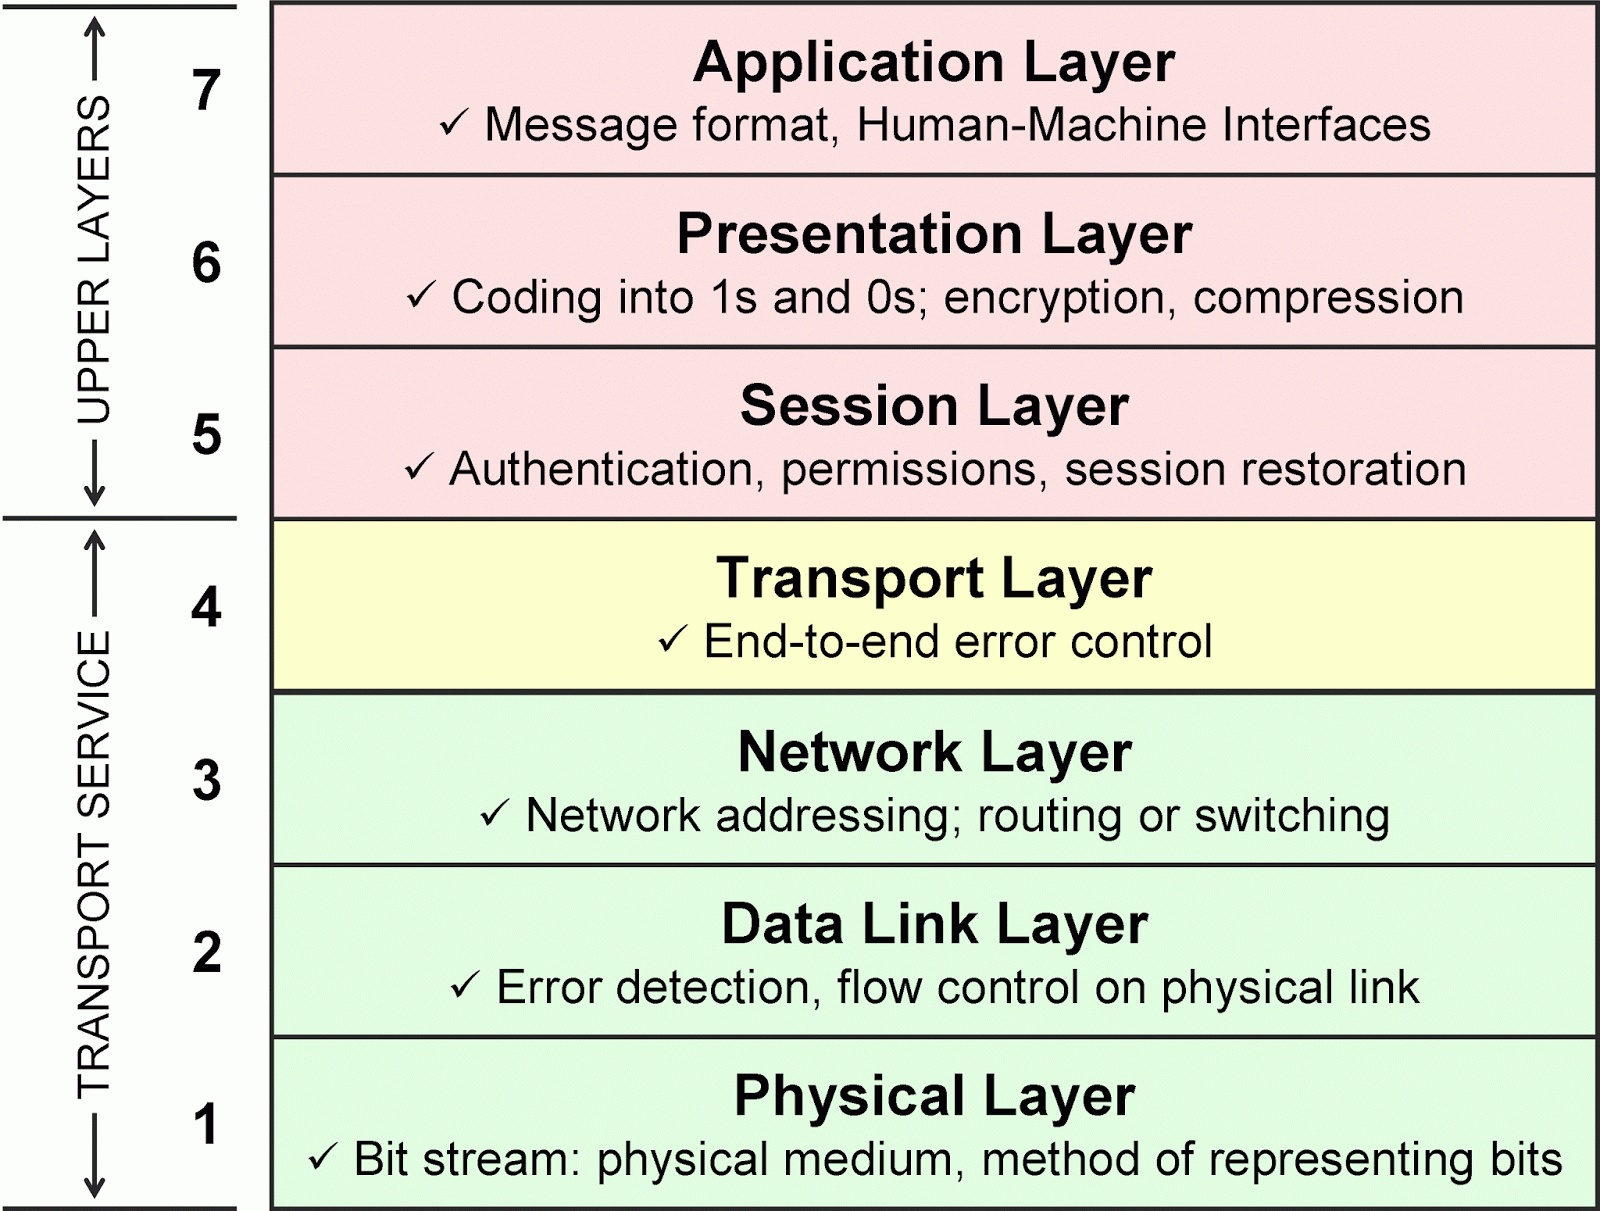
\includegraphics[width=0.7\textwidth]{figures/osi.png}
	\caption{\acf{osi} model \cite{Zikrillah}.}
	\label{fig:osi}
\end{figure}

This characteristics are what make this standard quite significant for \ac{iot}. Since \ac{iot} sensors and actuators have many battery constrains, using a protocol that has this facts in mind, make IEEE 802.15.4 a suitable standard for communications within \ac{wsn}s.

IEEE 802.15.4 is also the baseline for other \ac{iot} communication protocols such as ZigBee, which will be covered in a section below.


\subsubsection{6LoWPAN}
\acf{6plowpan} is a standard presented by Internet Engineering Task Force (IETF), and its main objective was to implement IPv6 over low power networks, granting the possibility for IoT devices to be reached through the Internet using a unique address. Also this would allow the use of some IPv6 important features such as Quality of Service (QoS), mobility and multicasting.

\ac{6plowpan} uses the previously addressed standard, IEEE 802.15.4, for the two lowest layers of the OSI model, shown in Figure \ref{fig:osi}. Since the network layer protocol was needed to comply with those two lower layers, and the requirements for an IPv6 based protocol didn't match the constrained IEEE 802.15.4 standard, 6LoWPAN implemented mechanisms to efficiently transport IPv6 packets within small link layer frames \cite{chalappuram2016}. 

In order to use \ac{6plowpan} in a IPv6 network, it is only needed a low complexity edge router to route the traffic from IPv6 to \ac{6plowpan}, as shown in Figure \ref{fig:6low}. 

\begin{figure}[H]
	\centering
	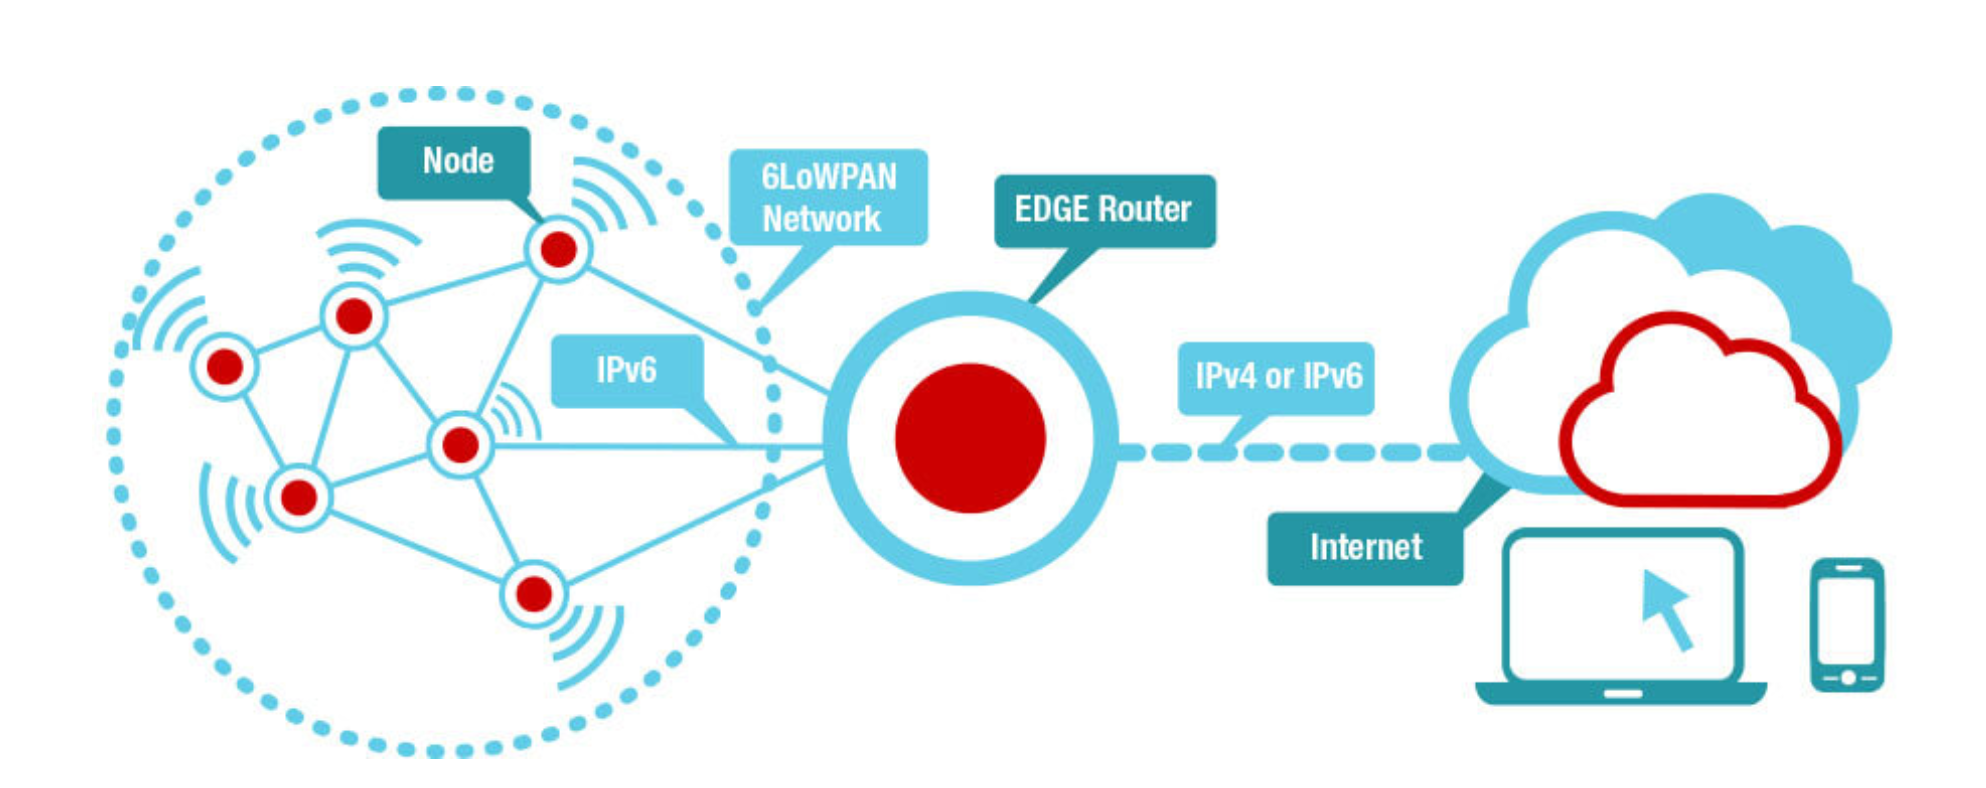
\includegraphics[width=0.7\textwidth]{figures/edge.png}
	\caption{Connection between a 6LoWPAN and an IPv6 network \cite{6low}.}
	\label{fig:6low}
\end{figure}


To sum up, with the proliferating market of \ac{iot} devices, the use of IPv6 is unavoidable, and the fact that 6LoWPAN offers a low power and low complexity way of addressing this problem, makes this protocol a viable solution for its use in \ac{iot} environments \cite{Mehboob2016}.  


\subsubsection{ZigBee}
ZigBee is a standard introduced by ZigBee Alliance, released to the public in June 2005. ZigBee is built on top of the IEEE 802.15.4 standard, addressed early, and it specifies the its own implementation of upper layers \cite{INSTEON2013}. As shown in Figure \ref{fig:zig}, ZigBee provides on the Application, a ZigBee Cluster Library (ZCL) that maps commands to be used by developers when defining application profiles.


\begin{figure}[H]
	\centering
	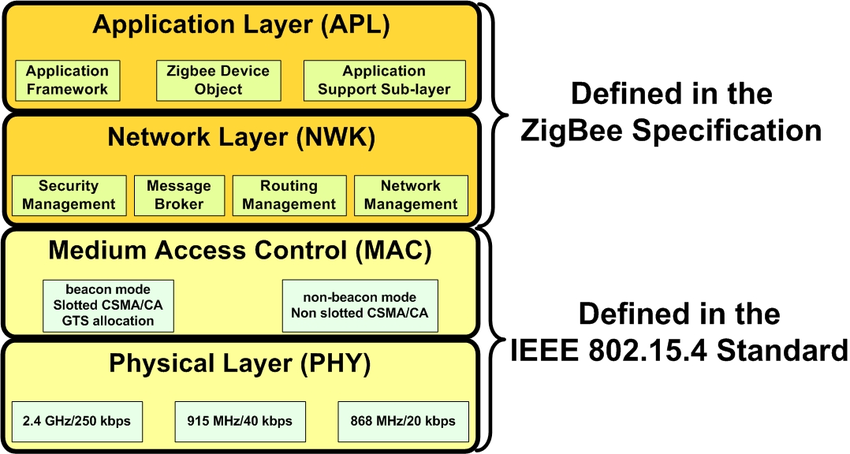
\includegraphics[width=0.7\textwidth]{figures/zig.jpg}
	\caption{ZigBee protocol stack \cite{article}.}
	\label{fig:zig}
\end{figure}


Although other standards have been emerging on the IoT constrained devices market, ZigBee widely dominates this market as it has been targeting it since the beginning, as a very low power and low latency standard.
Although ZigBee is not suitable for long ranges and has low data transfer speeds, a single master node is able to control 254 devices such as light bulbs and light switches \cite{Mehboob2016}. 
To sum up, ZigBee fulfils every expected requirements to be a strong competitor for the IoT communication standards.

\subsubsection{\acf{ble}}

\acf{ble} was created by Bluetooth SIG, in 2011, as a way to address the low power constrained devices that emerged with the rising growth of \ac{iot}. 


Although \ac{ble} followed the specifications of Bleutooth 4.0, there was no compatibility between them and so, BLE wouldn't be compatible with most of the widely adopted Bluetooth protocol that most smartphones and tablets used. This fact forced the emerging of two new classes of bluetooth devices: Bluetooth Smart and Bluetooth Smart Ready, as shown in Figure \ref{fig:ble1} \cite{Andersson2014}. The first one, known as single-mode device, is only capable of communicate using BLE, being used in sensors (presence sensor, temperature sensors, etc.) or other types of battery-operated and low processing accessories. The second, also known as dual-mode Bluetooth, is capable of communicating with both BLE devices and classic Bluetooth devices, being more suitable for smartphones, IoT gateways and other more powerful devices. 

\begin{figure}[H]
	\centering
	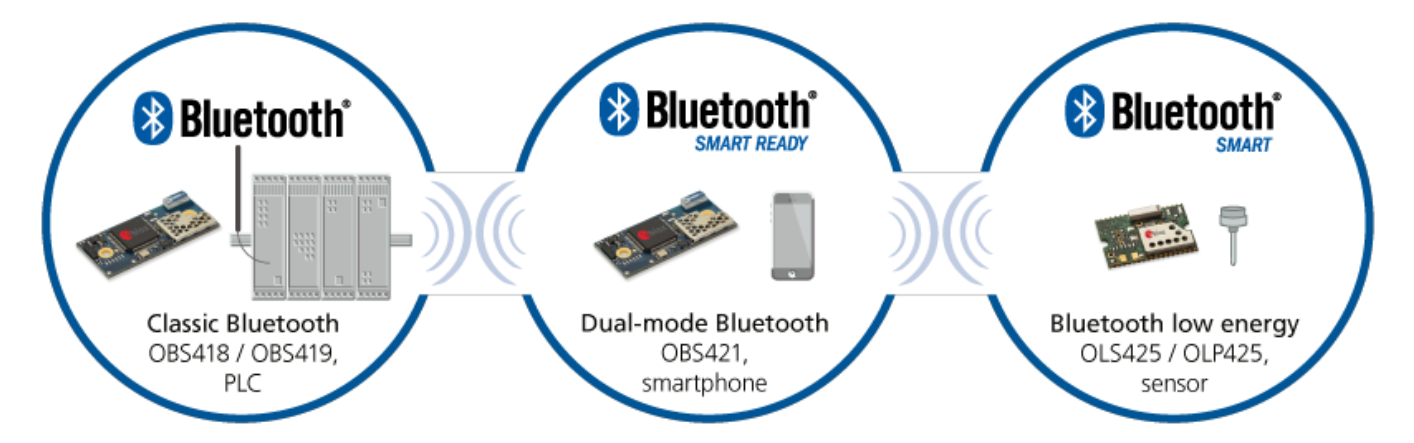
\includegraphics[width=0.9\textwidth]{figures/ble.png}
	\caption{Product examples of Bluetooth single and dual-mode modules. Adapted from \cite{Andersson2014}.}
	\label{fig:ble1}
\end{figure}

BLE is suitable to low-energy devices because it adopts a client/server model where devices are in a sleep state and periodically send advertisement messages for clients, such as a smartphone or a gateway, discover it and begin a connection as shown in Figure \ref{fig:ble2}. When connected, the clients can ask for data in a pre configured interval \cite{Andersson2014}. 

\begin{figure}[H]
	\centering
	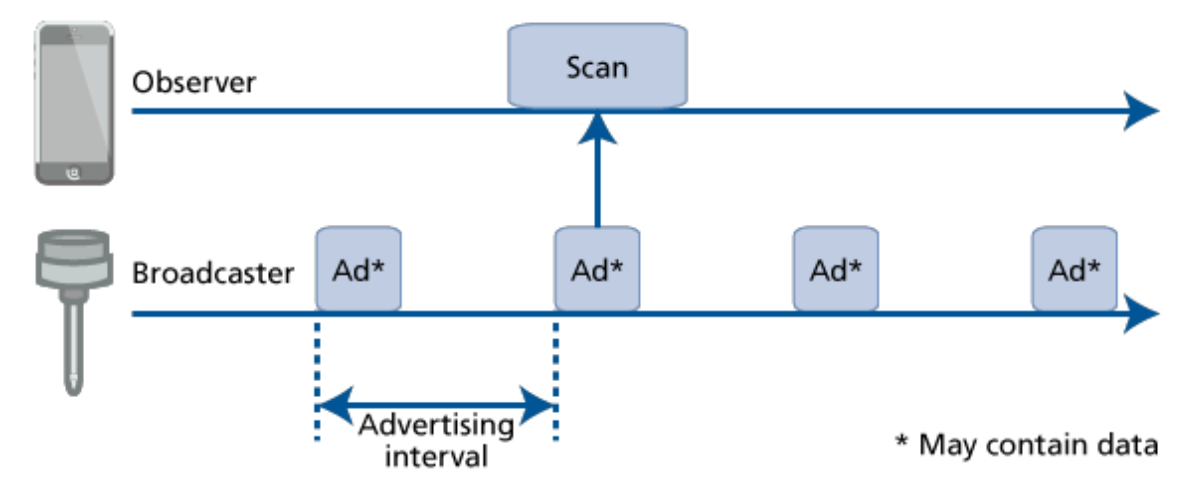
\includegraphics[width=0.9\textwidth]{figures/ble2.png}
	\caption{BLE discover of devices. Adapted from \cite{Andersson2014}.}
	\label{fig:ble2}
\end{figure}

To sum up, BLE is one of the best solutions for communications between IoT devices and gateways, since it offers low energy consumption and acceptable data transfer rates.

\subsubsection{Wireless Communication Protocols Comparison}
TODO  

\subsection{Application Protocols}

As previously stated, the fast growth of IoT devices motivated the search for lightweight protocols in order to enable this low resources devices to efficiently communicate with other nodes. 

In this section will be presented protocols that address the Application layer of the OSI model, shown in Figure \ref{fig:osi}, and are suitable to be used in \ac{iot}. Since \ac{iot} solutions address a huge amount of different scenarios, with different requirements, bellow will be presented protocols that have different features, and the strengths and weak points of each one will be evaluated.

\subsubsection{\acf{mqtt}}

\acf{mqtt} is a \ac{m2m} communication protocol introduced by IBM in 1999, but was only standardized in 2013 as OASIS \cite{Al-fuqaha2015}. \ac{mqtt} follows a publish/subscribe client/server model and, due to its simpleness, it is suitable to be used in constrained devices.

The publish/subscribe model features three components: a broker, publishers and subscribers. In the scenario shown on Figure \ref{fig:mqtt}, the central piece, the server, is a \ac{mqtt} Broker, and the other components such as data gatherers and data consumers are clients that connect to this broker. Clients are able to publish and/or subscribe to topics on the \ac{mqtt} Broker, and its task is to route messages from publishers, to the corresponding subscribers of each topic \cite{Al-fuqaha2015}. 

\begin{figure}[H]
	\centering
	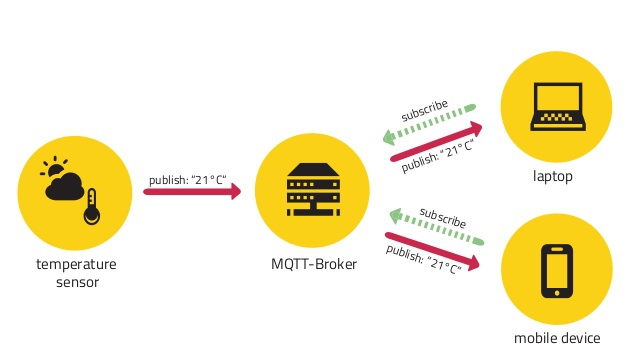
\includegraphics[width=0.9\textwidth]{figures/mqtt.jpg}
	\caption{MQTT protocol architecture \cite{Turan}.}
	\label{fig:mqtt}
\end{figure}

Taking as example the case illustrated in Figure \ref{fig:mqtt}, a temperature sensor publishes data on some topic and the \ac{mqtt} Broker forwards this messages to the clients subscribed to that temperature topic. MQTT offers the possibility of four different communication types: one-to-one,  many-to-one, one-to-many, many-to-many \cite{Chen2016}.The great advantage of this protocol is that publishers do not need to send the same information to every client nor need to be aware of its presence. This fact makes this protocol very suited to be used in contexts where devices need to be as efficient as possible, which is the case of \ac{iot} environments. 

Regarding the guarantees of a successful message delivery, MQTT has three levels of \acf{qos}: at most once (0), at least once (1) or exactly once (2) \cite{mqtt_qos}. The level 0 of \ac{qos}, also known as "Fire and Forget" is the most basic one, since the message is sent only one time to the subscribers. It has no fail mechanisms, so if, by a network error, the message do not reach its target, is not resented by the broker. This level of QoS is suited when occasional unsuccessfully message delivers do not jeopardy the system functioning or when the broker-clients connection is stable enough. With level 1 of \ac{qos}, the sender stores the published message in cache and waits for the acknowledge message. If the acknowledge is not received within a pre programmed time interval, the message is sent again. The drawback of this level os \ac{qos} is that a message can be received multiple times if the acknowledge do not reach the sender. Lastly, \ac{qos} level 2 grants that a message is delivered exactly one time, however this process introduces a greater overhead, as it takes longer that any other level of \ac{qos}.

Other important features of MQTT are the last will message, where a client can register a message to be delivered to a specific topic in the case of a lost of connection between the broker and the client, and the security concerns, in which an authentication method is provided, using a username and password. Also, regarding security, the payload of the message can be encrypted with SSL/TLS.

To sum, MQTT is an important Application layer protocol and very suitable to be used in constrained networks and devices as a powerful communications standard.

\subsubsection{\acf{coap}}

\acf{coap} is an application protocol created by IETF with the objective of providing \acf{rest} functionalities to constrained devices and networks. \ac{rest} is a standard used to communications between computer systems on the Internet. Although this protocol its a well known and adopted standard for HTTP, when talking about IoT, whose devices are very constrained energy-wise, this standard presents too much of an overhead \cite{Salman2013}. \ac{coap} comes to resolve this drawback by presenting a lightweight RESTful solution, following a request/response pattern, with the constrained devices market in mind.

As shown in Figure \ref{fig:coap}, \ac{coap}, unlike HTTP, uses \ac{udp} in the underlying layer of its architecture. This fact makes \ac{coap} communication more efficient as packets are sent without handshaking, or congestion control mechanisms that would introduce more overhead, used by TCP. The communication reliability is implemented by \ac{coap} lightweight internal mechanisms \cite{Salman2013}.

\begin{figure}[H]
	\centering
	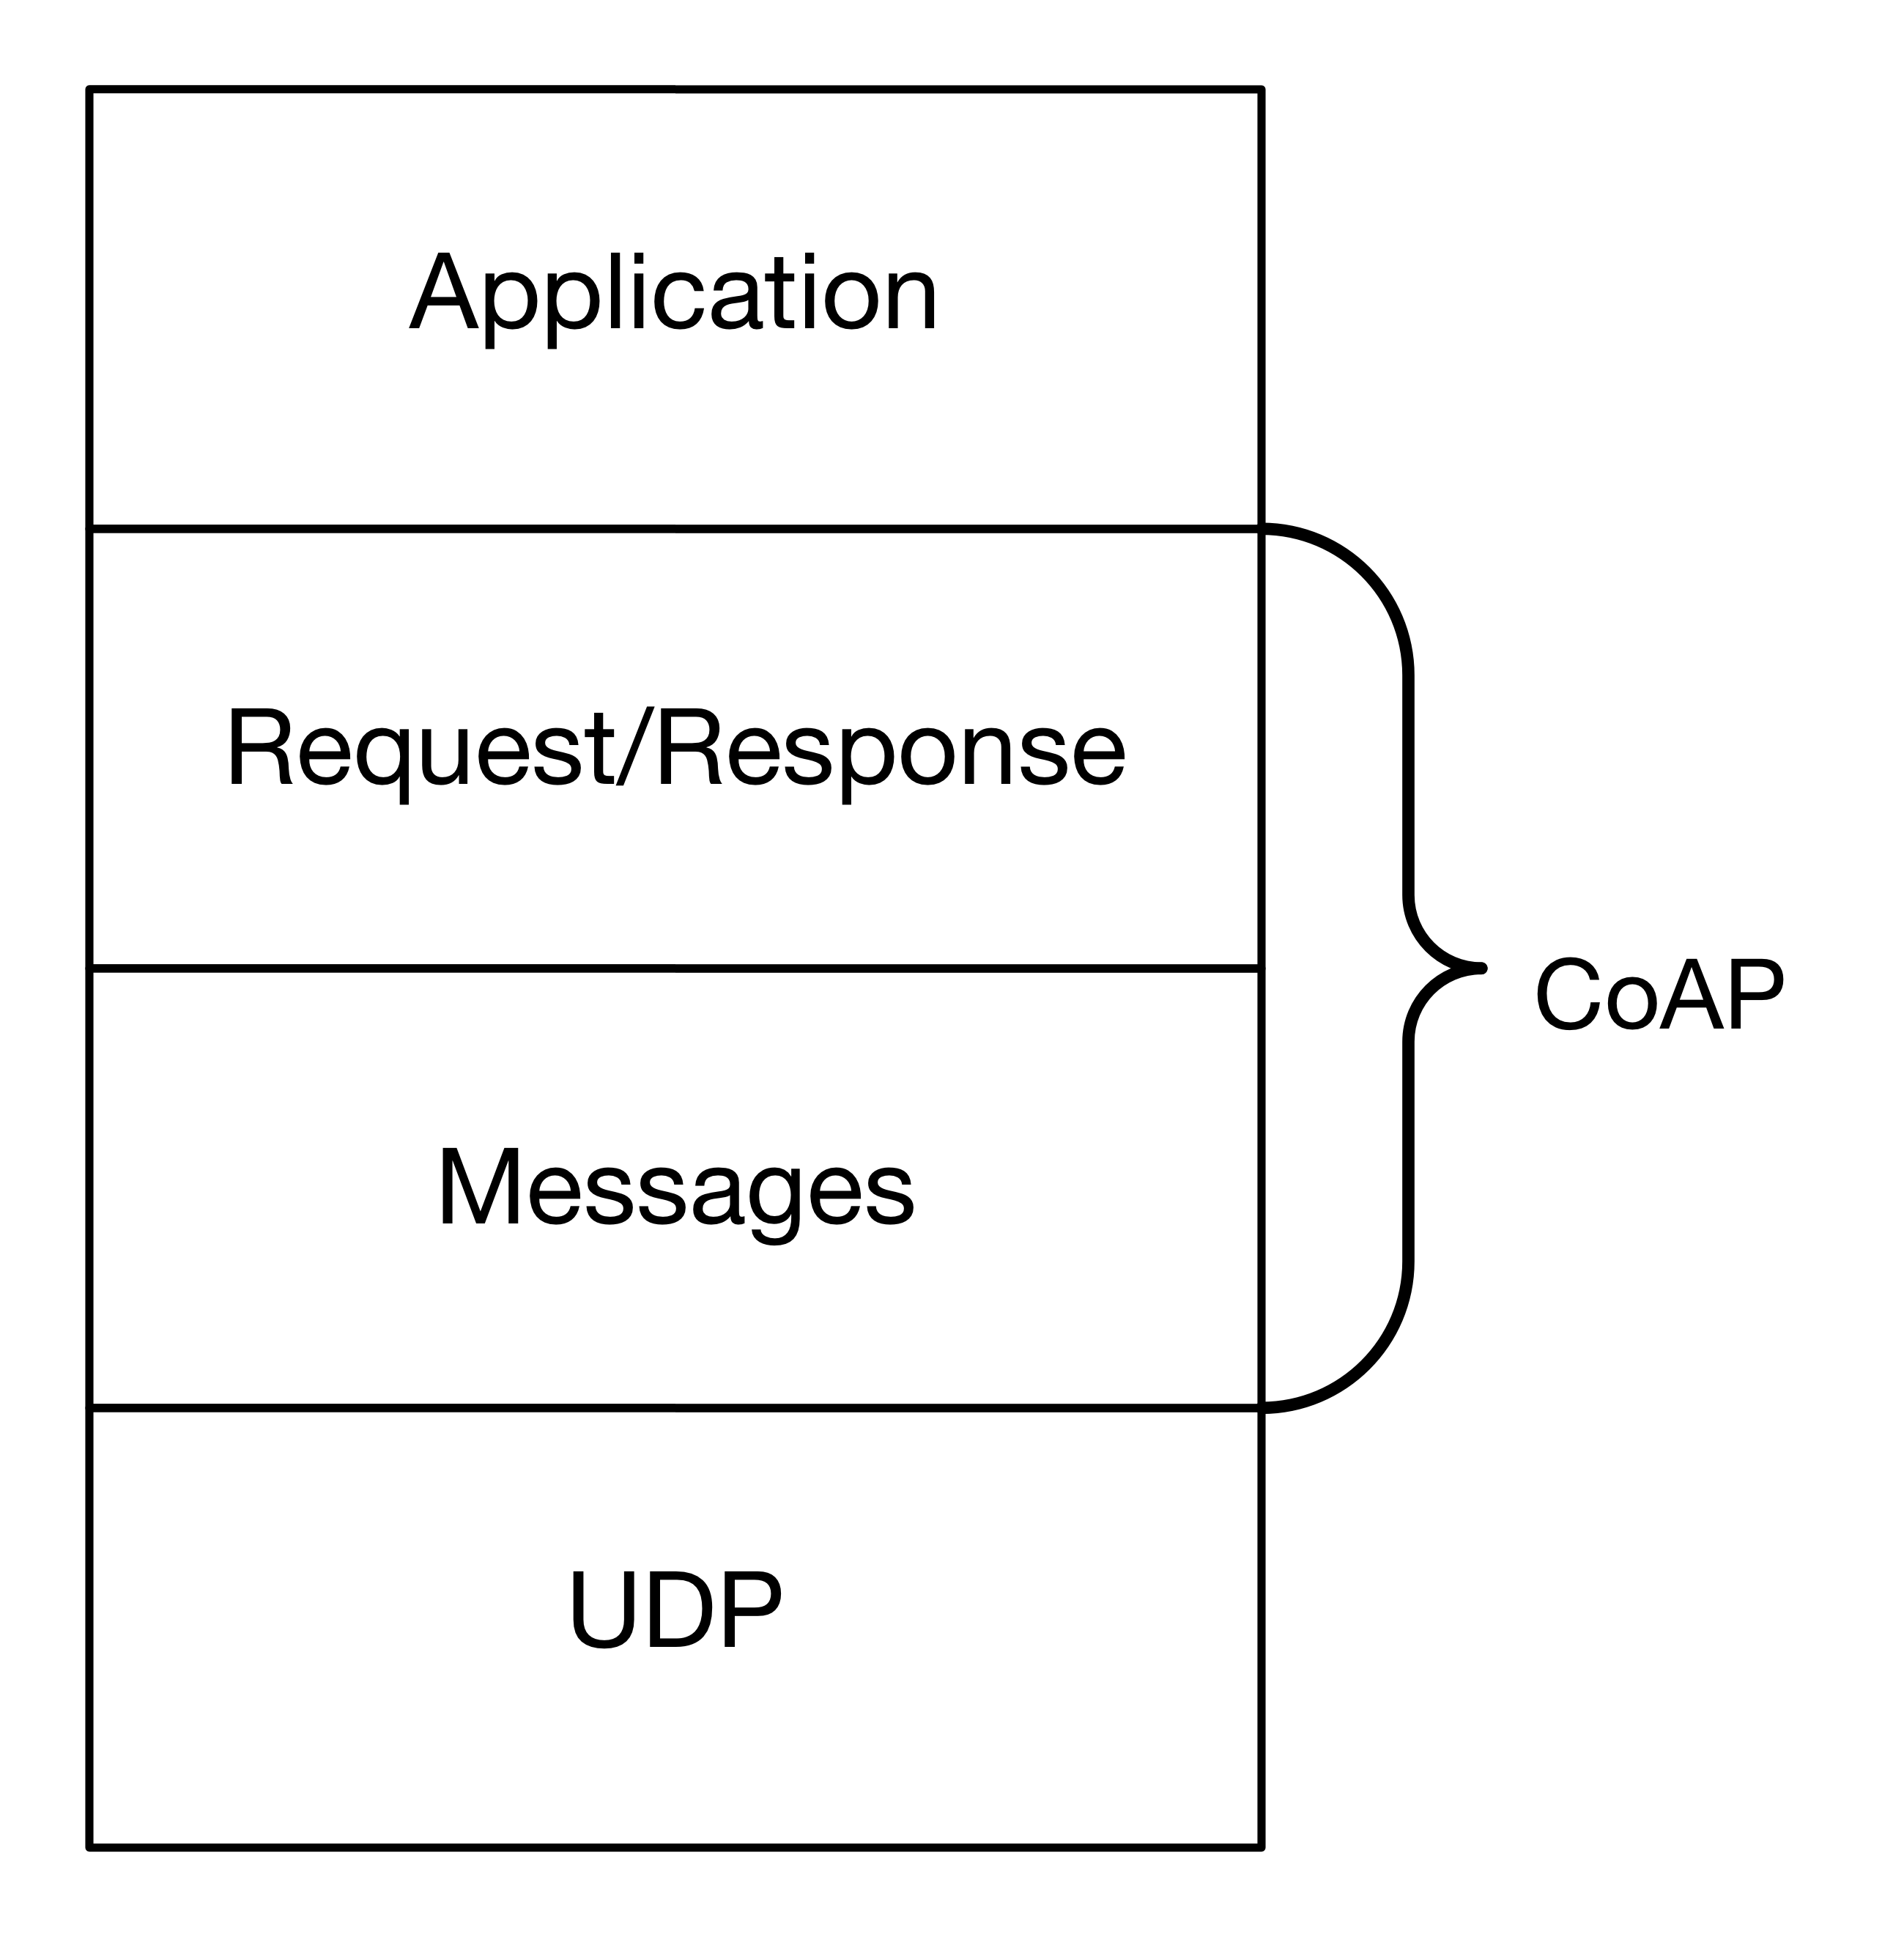
\includegraphics[width=0.9\textwidth]{figures/coap.png}
	\caption{\ac{coap} protocol architecture \cite{Mehboob2016}.}
	\label{fig:coap}
\end{figure}

As is also shown in Figure \ref{fig:coap}, \ac{coap} is divided into two sub-layers: request/response and messages. The messages layer is responsible for message processes such as fail and duplication handling, since UDP, as stated before, do not have reliability mechanisms \cite{Salman2013}. The request/response layer is responsible for enable the RESTful interaction by offering well known methods such as GET, POST, PUTT and DELETE to interchange data \cite{Lerche2012}.

\ac{coap} has also an "observe" resource that enables clients, through a publish/subscribe mechanism, to observe a resource and when there is a change, the client is notified by the server \cite{Lerche2012}. All \ac{coap} features make this protocol also very attractive for some use cases in an \ac{iot} environment.


\subsubsection{\acf{amqp}}

\acf{amqp} is a communication protocol, initially created aiming the financial sector, that, like \ac{mqtt}, runs over \ac{tcp} and adopts a publish/subscribe architecture. The use of this protocol for financial purposes is due to the fact that \ac{amqp} has powerful mechanisms that grant high reliability and scalability that are crucial for that sector.

\ac{amqp} architecture is composed, as shown in Figure \ref{fig:amqp} by three elements: producers, clients and the broker, being the last one divided by two components, the exchange and topic queues. The producers publish messages in a specific topic and the exchange module is responsible for deposit that messages in the correct topic queue. Clients are connected to the queues of specific topics and then have access to the published messages in that queues \cite{Salman2013}. This system allows that instead of the broker having to send the same message to multiple clients subscribed to a topic, the message is only sent to the respective queue. Also, it allows clients to be offline at the time the message is sent to the queue, since it becomes stored there until it is consumed \cite{Al-fuqaha2015}.

\begin{figure}[H]
	\centering
	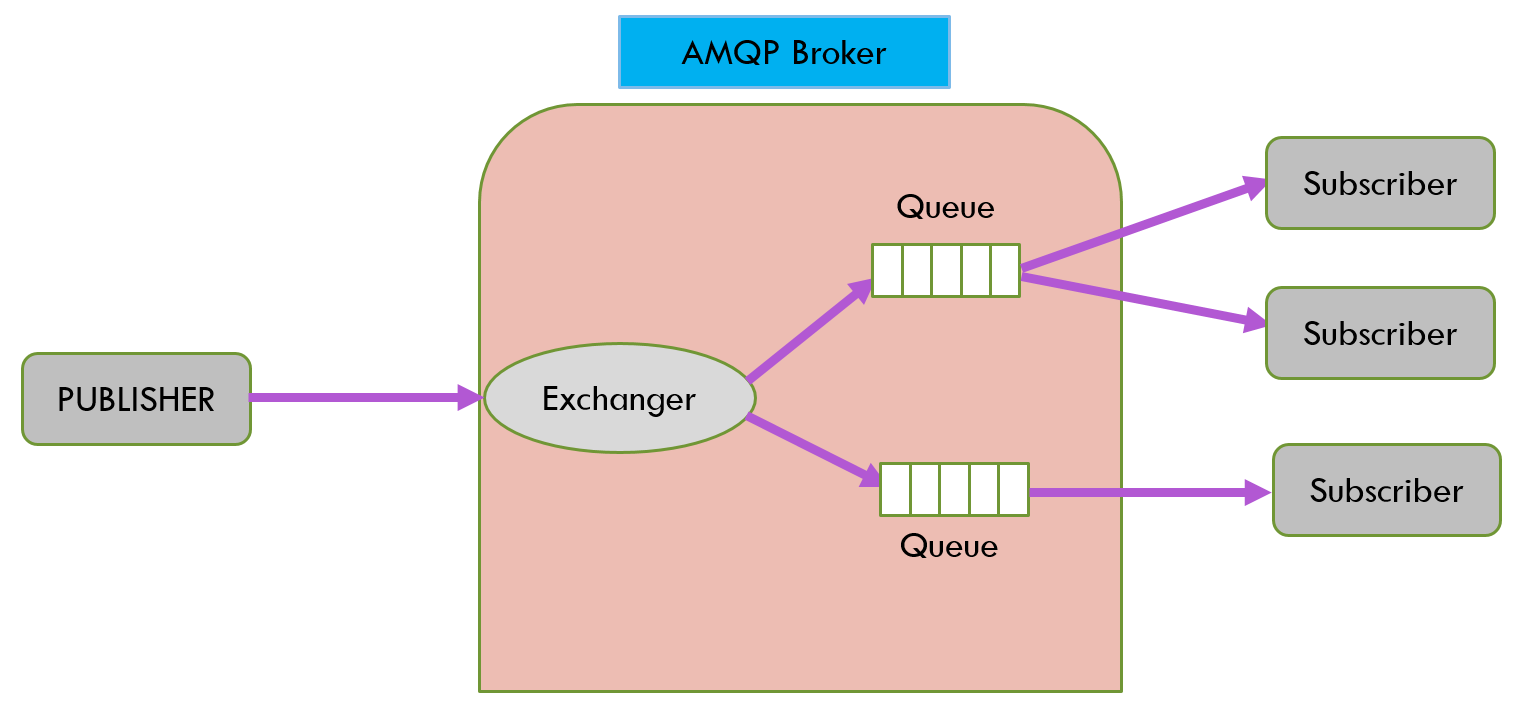
\includegraphics[width=0.9\textwidth]{figures/amqp.png}
	\caption{\ac{amqp} protocol architecture \cite{Badugu}.}
	\label{fig:amqp}
\end{figure}

Although for majority of \ac{iot} environments reliability is not a deciding feature for the communication system, there are some few cases where that is indispensable. For instance, in a situation where a luminance sensor that sends periodic data of the measured values, a lost message will not be a huge problem because shortly after, another value will be sent and the prior loss will have almost no impact to the system. However in a hospital, if an emergency message in not delivered successfully could mean a life threatening situation for a patient. Situations like this ensure the importance of a communication protocol like \ac{amqp} in the \ac{iot} context.

\subsubsection{\acf{xmpp}}

\acf{xmpp} is, like the former, a standardized message-oriented communication protocol and it was created by Jabber open-source community in 1999 for establish near real-time instant messaging (IM), presence information, and others \cite{Badugu}.

\ac{xmpp}, as shown in Figure \ref{fig:xmpp} uses a decentralized architecture where there can be more than one server and the messages can be transferred between them until they reach the desired destination, ensuring that way a high scalability \cite{Al-fuqaha2015}.

\begin{figure}[H]
	\centering
	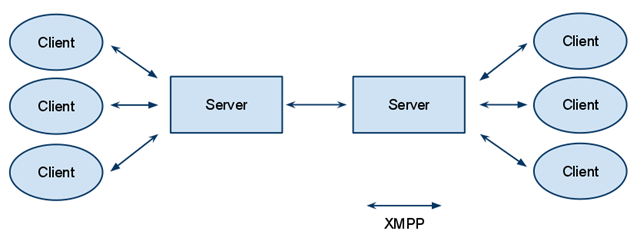
\includegraphics[width=0.9\textwidth]{figures/xmpp.png}
	\caption{\ac{xmpp} protocol architecture \cite{Adafruit}.}
	\label{fig:xmpp}
\end{figure}

Salman2013
Unlike the protocols addressed previously, \ac{xmpp} supports not only a publish/subscribe architecture, but also a request/response one, however, by using \ac{xml} messages that, although providing a greater flexibility, induce a higher overhead than the former protocols, which creates more power consumption for devices \cite{Salman2013}. Fact that can be a problem for \ac{iot} environments, as stated before.

Although \ac{xmpp} has some drawbacks, it still has capacity to be an important protocol in some specific \ac{iot} use cases, due to the near real time message exchanging and the high extensibility offered.

\subsubsection{Interaction Protocols Comparison}

In this chapter, the protocols previously addressed will be compared and will be provided an evaluation of the environments where each one of them is more suitable. Bellow in Table \ref{iotapplayer}, the protocols are compared based on the type of transport used, the presence of security mechanisms and \ac{qos}, and also the support of Publish/Subscribe or Request/Response patterns.

\begin{table}[]
	\centering
	\begin{tabular}{|l|l|l|l|l|}
		\hline
		& \textbf{MQTT}              & \textbf{CoAP} & \textbf{AMQP} & \textbf{XMPP} \\ \hline
		\textbf{Transport}         & TCP                        & UDP           & TCP           & TCP           \\ \hline
		\textbf{Security}          & SSL and User/Password auth & DTLS          & SSL           & SSL           \\ \hline
		\textbf{QoS}               & Yes                        & Yes           & Yes           & No            \\ \hline
		\textbf{Publish/Subscribe} & Yes                        & No            & Yes           & Yes           \\ \hline
		\textbf{Request/Response}  & No                         & Yes           & No            & Yes           \\ \hline
	\end{tabular}
	\caption{IoT Application Protocols Comparison.}
	\label{iotapplayer}
\end{table}

Regarding \ac{mqtt} and \ac{amqp}, both protocols use a publish/subscribe pattern but, although \ac{amqp} offers a wider variety of features, \ac{mqtt} gains for being more lightweight, simpler and easier to deploy in most cases, client and broker wise. For this fact, \ac{mqtt} is usually the choice for most systems, where there are not very restrictive requirements. Nevertheless, both protocols are suited for \ac{iot} environments with constrained and low-power devices.

Looking at \ac{coap}, the greater difference between the last two is the use request/response pattern, instead of a publish/subscribe one. Also, \ac{coap} uses a one-to-one transfer protocol between a client and a server, which makes it more suitable as state change model, instead of a event driven one.

Finally, the \ac{xmpp} although being the protocol with the most extensive number of features, such as allowing both publish/subscribe and request/response patterns, and being a near real time communication protocol, still lacks by not being as lightweight as the other protocols. Nevertheless, this protocol has a place in the market, for solutions where reliability is a key factor.

\subsection{Fault-Tolerance in IoT}



As addressed in the sections above, \ac{wsn}s allied to \ac{iot} principles enabled the appearance of smart environments constituted by networks of sensors, gateways and automation components. However in such systems, a failure in a component can put in jeopardy the whole system and, therefore, there is a need to implement proper fail recovery mechanisms to avoid irreversible failures.

In the typical smart environments, sensors and actuators are connected to a gateway, also called a sink, that is capable of communicate with them and, either process itself the received data or send it to other component responsible for doing so \cite{Gia2015}. Therefore, three core components, of a smart environment, that have a direct effect on the whole system functioning, can be considered: devices, gateways and automation engines. A device malfunctioning can only be surpassed by human intervention since it has no self healing mechanisms. Otherwise there would have to be redundant devices. At the gateways level, since it is a sink device, where the information flows to, there would be also necessary redundant gateways or, in case of multiple gateways connected to different devices, the other gateways should be able to sense that there was a disconnected gateway and takeover the control for the lost devices. Lastly, the automation engines, like the other components, could resolve a failure situation by having redundancy or self healing techniques implemented in the application. However, in case of irreversible failure, gateways should be able to sense that the automation components are unreachable and, in a perfect scenario, having automation logic implemented so that the system could work at an emergency state until the automation engines were re-established.

\subsection{\ac{iot} enabled \ac{bas} solutions}

According to the author of \cite{TransformativeWave}, the old industry of \ac{bas}s systems is being disrupted by the Internet of Things. Only some of the most known \ac{bas} companies are trying to a integrate \ac{iot} principles and open protocols in their solutions in order to maintain themselves in the market. The emerge of cheap and small devices with wireless connectivity using open standards and the possibility of creating affordable automation environments, using open-source software, are now at reach, providing a wider variety of solutions to empower buildings with automation capability's and thus, reduce the energy consumption while increasing the comfort in buildings.

A practical example of a building automation system, using \ac{iot} principals and standards, is HCL Technologies \ac{bas}. HCL Technologies is a member of the Intel Internet of Things Solutions Alliance \cite{intel} and uses an Intel-based gateway to deliver a powerful, yet cost-effective building management solution \cite{hcl}. In this system, as shown in Figure \ref{fig:intel}, is used an Intel's \ac{iot} gateway empowered with HCL \ac{bas} software, which is responsible for providing a web interface and means for simple automation mechanisms such as, per example, turning air conditioners on when some temperature threshold is reached. The HCL \ac{bas} software and gateway supports protocols like ZigBee and Wi-Fi, and the translation between them is made without building manager's intervention.


\begin{figure}[H]
	\centering
	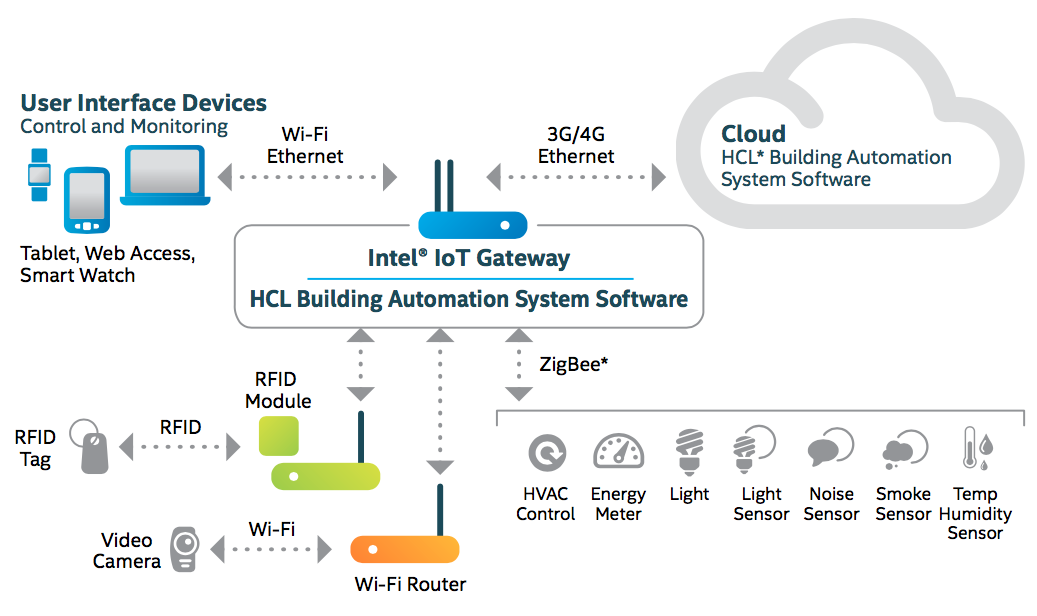
\includegraphics[width=0.9\textwidth]{figures/intelhclarch.png}
	\caption{HCL Technologies \ac{bas} deployment architecture \cite{hcl}.}
	\label{fig:intel}
\end{figure}

Although the presented solution constitutes a robust and state of the art solution as a \ac{bas}, with basic automation that can address most of building managers needs, there is a lack of complex automatic correlations between events generated by the sensors network. In the next section will be presented the importance of \acf{cep} modules to enhance the performance of event processing as well as the intelligence of a building through complex correlations.


\section{Automation Logic}
Automation can be described as actions preformed without human intervention. In the present dissertation context, automation is achieved using a logic component that receives all events, gathered by sensors from the environment, and infer actions based on buildings manager preloaded rules. For instance, events like movement in a room or temperature and humidity changes, are sent to this automation component that, based on the rules, can send triggers to turn on/off lights, air conditioners or others.

In a small house, the number of sensors and events are fairly small and thus, there is no need for a powerful and complex automation unit. However, in a building context, the amount of events generated is much higher, which requires the use of a more efficient and high performance platform. Also in an environment with so many variables, events cannot be treated isolated from the greater context, so there is a need for a platform that can be able to correlate this isolated events and infer more complex actions.

In the next subsection, will be presented a system capable of infer actions based on the processing and correlation of large event streams.

\subsection{\acf{cep}}

With the emergence of \ac{iot} in different areas, huge amounts of data, that need proper analysis, are produced. However, in areas like smart homes and buildings, the information streams need to be processed almost instantly in order to infer quick actions. \acf{cep} is a technology used to process and analyse large streams of data, from multiple sources, and infer real-time conclusions or actions based on the detection of patterns and complex events. As illustrated in Figure \ref{fig:cep}, a complex event is inferred when a certain number of isolated events happen in specific conditions.  


\begin{figure}[H]
	\centering
	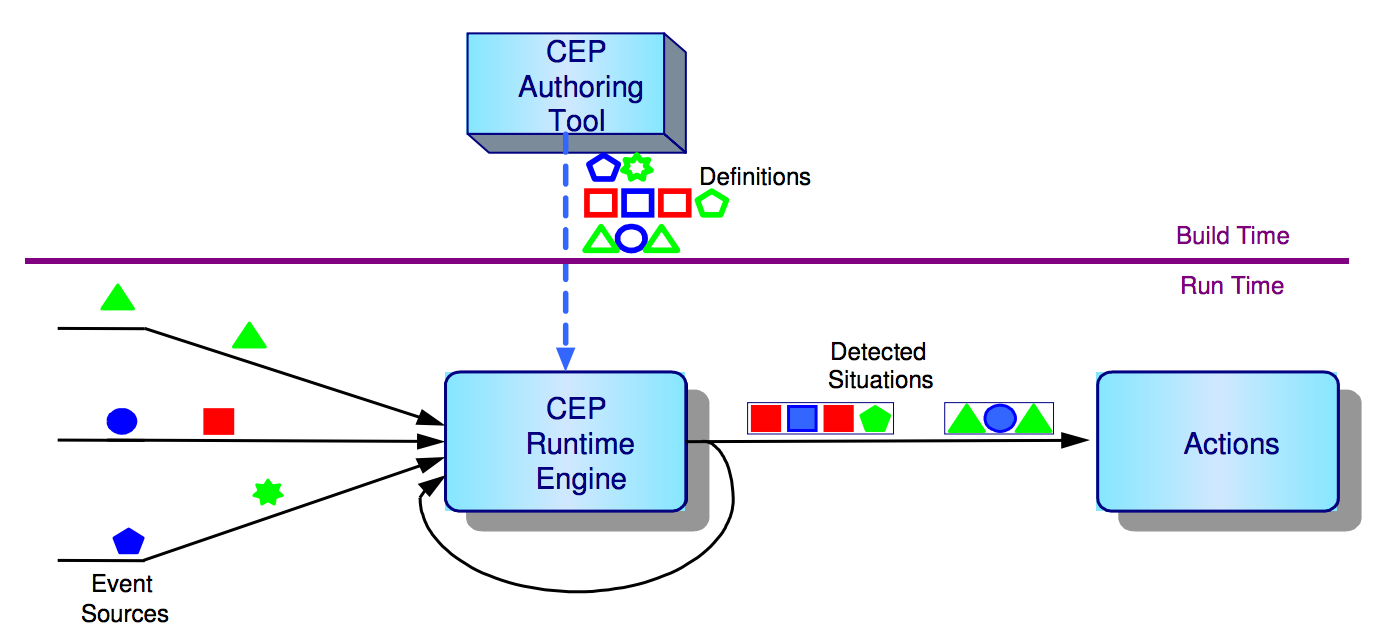
\includegraphics[width=0.9\textwidth]{figures/cep1.png}
	\caption{Detection of complex events using Complex Event Processing \cite{Pooja2015}.}
	\label{fig:cep}
\end{figure}

This automation technology is used in different contexts where, a real-time and high performance platform to process data, is needed. One of this cases is the financial industry where, in order to take low risk and profitable actions, \ac{cep} is used to deduce real-time trading predictions.


As stated before, smart buildings could also use the \ac{cep} technology to greatly increase the quality of its automation. For instance, with a \ac{cep} engine, the events generated by the network of sensors could be processed by this component to preform actions that, with a classic automation system, would be impossible. As a simple example, in an empty room where the air conditioner is turned off, a great decrease of temperature over a small period of time could mean that a window was left open and thus, a message could be sent to the building manager alerting this situation. In this example, with the gathered data from different sensors, such as temperature and presence, over some time, the \acf{cep} engine was able to infer a conclusion. This type of conclusions are only achieved if the automation system has in consideration multiple events across time and do not simply analyse them separately.

A \ac{cep} engine implements a set of tools such as filtering, time windowing, aggregation or pattern detection of events, and make possible to design complex rules using this mechanisms. They can be implemented either by using a query-based model using a query language similar to SQL, or a rule-based model, where a rule is divided in three components: an event, the condition that is evaluated when the event arrives and the action that is taken when the condition is satisfied.



